% Source-SHA256: 397cd2ee2b9a3076028422a9f010a565cbccb1973ff6baabe7ee0b1bca1b30f7
% !TeX program = xelatex
\documentclass[a4paper,11pt]{article}
\usepackage{fontspec}
\IfFontExistsTF{TeX Gyre Pagella}{\setmainfont{TeX Gyre Pagella}}{\setmainfont{P052}}
\IfFontExistsTF{TeX Gyre Heros}{\setsansfont{TeX Gyre Heros}}{\setsansfont{Nimbus Sans}}
\IfFontExistsTF{TeX Gyre Cursor}{\setmonofont{TeX Gyre Cursor}[Scale=0.88]}{\setmonofont{Nimbus Mono PS}[Scale=0.88]}
\usepackage{babel}
\babelprovide[import,main]{spanish}
\usepackage{microtype}
\usepackage[a4paper,margin=2.4cm,headheight=23pt,headsep=10pt,footskip=1.1cm]{geometry}
\raggedbottom
\setlength{\emergencystretch}{3em}
\hyphenpenalty=10000
\exhyphenpenalty=10000
\clubpenalty=10000
\widowpenalty=10000
\usepackage{xcolor}
\definecolor{navybg}{HTML}{0B1D2E}
\definecolor{navydeep}{HTML}{123049}
\definecolor{lightblue}{HTML}{8FD3FE}
\definecolor{amber}{HTML}{F5A623}
\definecolor{softgray}{HTML}{5B6570}
\usepackage{titlesec,needspace}
\setcounter{secnumdepth}{-1}
\setcounter{tocdepth}{2}
\titleformat{\section}{\sffamily\Large\bfseries\color{navydeep}\raggedright}{}{0pt}{}
\titleformat{\subsection}{\sffamily\large\bfseries\color{navydeep}\raggedright}{}{0pt}{}
\titlespacing*{\section}{0pt}{20pt}{9pt}
\titlespacing*{\subsection}{0pt}{14pt}{6pt}
\usepackage{fancyhdr}
\pagestyle{fancy}
\fancyhf{}
\fancyhead[L]{\small\sffamily\color{softgray}Compás a compás}
\fancyhead[R]{\small\sffamily\color{softgray}Manual de uso}
\fancyfoot[L]{\small\sffamily\color{softgray}Aplicación 0.7.0 · 18/10/2026}
\fancyfoot[R]{\small\sffamily\color{softgray}\thepage}
\renewcommand{\headrulewidth}{0.4pt}
\usepackage{array,longtable,booktabs,calc}
\newcounter{none}
\renewcommand{\arraystretch}{1.15}
\usepackage{enumitem}
\setlist[itemize]{leftmargin=1.4em,itemsep=3pt,topsep=5pt}
\setlist[enumerate]{leftmargin=1.8em,itemsep=3pt,topsep=5pt}
\usepackage{fvextra,framed,seqsplit}
\fvset{fontsize=\small,breaklines=true,breakanywhere=true,frame=leftline,framerule=1.4pt,rulecolor=\color{lightblue},framesep=8pt}
\RecustomVerbatimEnvironment{verbatim}{Verbatim}{breaklines,breakanywhere,samepage=true,fontsize=\small}
\let\originaltexttt\texttt
\renewcommand{\texttt}[1]{\originaltexttt{\seqsplit{#1}}}
\providecommand{\tightlist}{\setlength{\itemsep}{2pt}\setlength{\parskip}{0pt}}
% Pandoc 3.2+ envuelve las imágenes en \pandocbounded; con versiones anteriores no existe y esta definición no cambia nada.
\providecommand{\pandocbounded}[1]{#1}
\usepackage{graphicx,xurl,tikz}
\usepackage[section]{placeins}
\usepackage{amssymb,newunicodechar}
\usepackage[colorlinks=true,linkcolor=navydeep,urlcolor=navydeep,pdftitle={Compás a compás - Manual de uso},pdfauthor={Jesús Quevedo Rodríguez}]{hyperref}
\usepackage{bookmark}
\newunicodechar{♭}{\texorpdfstring{\ensuremath{\flat}}{\unichar{9837}}}
\newunicodechar{♯}{\texorpdfstring{\ensuremath{\sharp}}{\unichar{9839}}}
\newunicodechar{✓}{\texorpdfstring{\ensuremath{\checkmark}}{\unichar{10003}}}
\newunicodechar{✗}{\texorpdfstring{\ensuremath{\times}}{\unichar{10007}}}
\newunicodechar{→}{\texorpdfstring{\ensuremath{\rightarrow}}{\unichar{8594}}}
\newunicodechar{←}{\texorpdfstring{\ensuremath{\leftarrow}}{\unichar{8592}}}
\setlength{\parindent}{0pt}
\setlength{\parskip}{6pt}
\renewcommand{\topfraction}{0.95}
\renewcommand{\bottomfraction}{0.95}
\renewcommand{\textfraction}{0.05}
\renewcommand{\floatpagefraction}{0.6}
\setcounter{topnumber}{3}
\setcounter{totalnumber}{4}
\begin{document}
\begin{titlepage}
\newgeometry{margin=0cm}
\thispagestyle{empty}
\pagecolor{navybg}
\color{white}
\vspace*{3cm}
\begin{center}
{\sffamily\bfseries\fontsize{16}{19}\selectfont\color{amber} COMPÁS A COMPÁS\par}
\vspace{1cm}
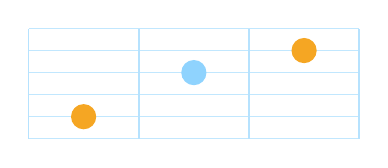
\begin{tikzpicture}[x=0.7cm,y=0.28cm]
\foreach \y in {0,...,5} {\draw[lightblue!55,line width=0.5pt] (-3,\y)--(3,\y);}
\foreach \x in {-3,-1,1,3} {\draw[lightblue!65,line width=0.6pt] (\x,0)--(\x,5);}
\fill[amber] (-2,1) circle[x radius=0.16cm,y radius=0.16cm];
\fill[lightblue] (0,3) circle[x radius=0.16cm,y radius=0.16cm];
\fill[amber] (2,4) circle[x radius=0.16cm,y radius=0.16cm];
\end{tikzpicture}\par
\vspace{1.4cm}
{\sffamily\bfseries\fontsize{30}{38}\selectfont Manual de uso\par}
\vspace{0.8cm}
{\sffamily\fontsize{14}{20}\selectfont\color{lightblue} Editar, guardar e imprimir hojas de acordes\par}
\vfill
{\sffamily\small Autor del proyecto: Jesús Quevedo Rodríguez\par}
{\sffamily\small Aplicación 0.7.0 · 18/10/2026\par}
{\sffamily\small Repositorio: a01653/Compas-a-compas\par}
\vspace{2cm}
\end{center}
\end{titlepage}
\nopagecolor
\restoregeometry
\setcounter{page}{2}
\tableofcontents
\newpage
Aplicación 0.6.0 · Edición del manual: 17/10/2026. Autor del proyecto:
Jesús Quevedo Rodríguez.

\Needspace{3.5cm}
\hypertarget{preparar-una-canciuxf3n}{%
\section{Preparar una canción}\label{preparar-una-canciuxf3n}}

El botón \textbf{Manual} (icono de libro) de la barra superior abre una
página de ayuda en otra pestaña, con un resumen y un enlace a este
manual en PDF. Funciona igual en local que en GitHub Pages. Solo existe
en la aplicación: no aparece en los HTML ni en los PDF de canciones que
exportes.

\begin{enumerate}
\def\labelenumi{\arabic{enumi}.}
\tightlist
\item
  Abre la aplicación en
  \href{https://a01653.github.io/Compas-a-compas/}{GitHub Pages} o con
  \texttt{Abrir-Compas.cmd} desde la carpeta del proyecto. En local,
  conserva abierta la consola que arranca el servidor.
\item
  Abre el menú superior de tres puntos y pulsa \textbf{Nueva canción}, o
  pulsa \textbf{Abrir} para continuar una canción guardada. Para
  practicar puedes abrir \texttt{examples/cancion-demo.json}.
\item
  Pulsa el título de la cabecera para abrir los datos y escribe el
  \textbf{nombre de la canción} y la \textbf{tonalidad}. La tonalidad
  aparece a continuación del nombre en cada hoja. Puedes elegir su
  calidad para el color inicial de las franjas de las tarjetas. La
  \textbf{versión del documento} es una etiqueta opcional para tus
  revisiones; no cambia la versión de la aplicación.
\item
  Añade compases y sus posiciones. Revisa el resultado a la derecha y
  guarda con \textbf{Guardar JSON}.
\end{enumerate}

La interfaz tiene un editor compacto a la izquierda y la hoja a la
derecha. Los selectores de compás y tarjeta evitan listas verticales
largas. Digitación y grados quedan en la parte alta del editor; los
textos y la tonalidad de la tarjeta aparecen debajo. El editor conserva
desplazamiento interno cuando no cabe todo. En móvil se apilan las
zonas. \textbf{Ajustar al ancho} y los botones de zoom solo cambian la
vista, no el tamaño de impresión.

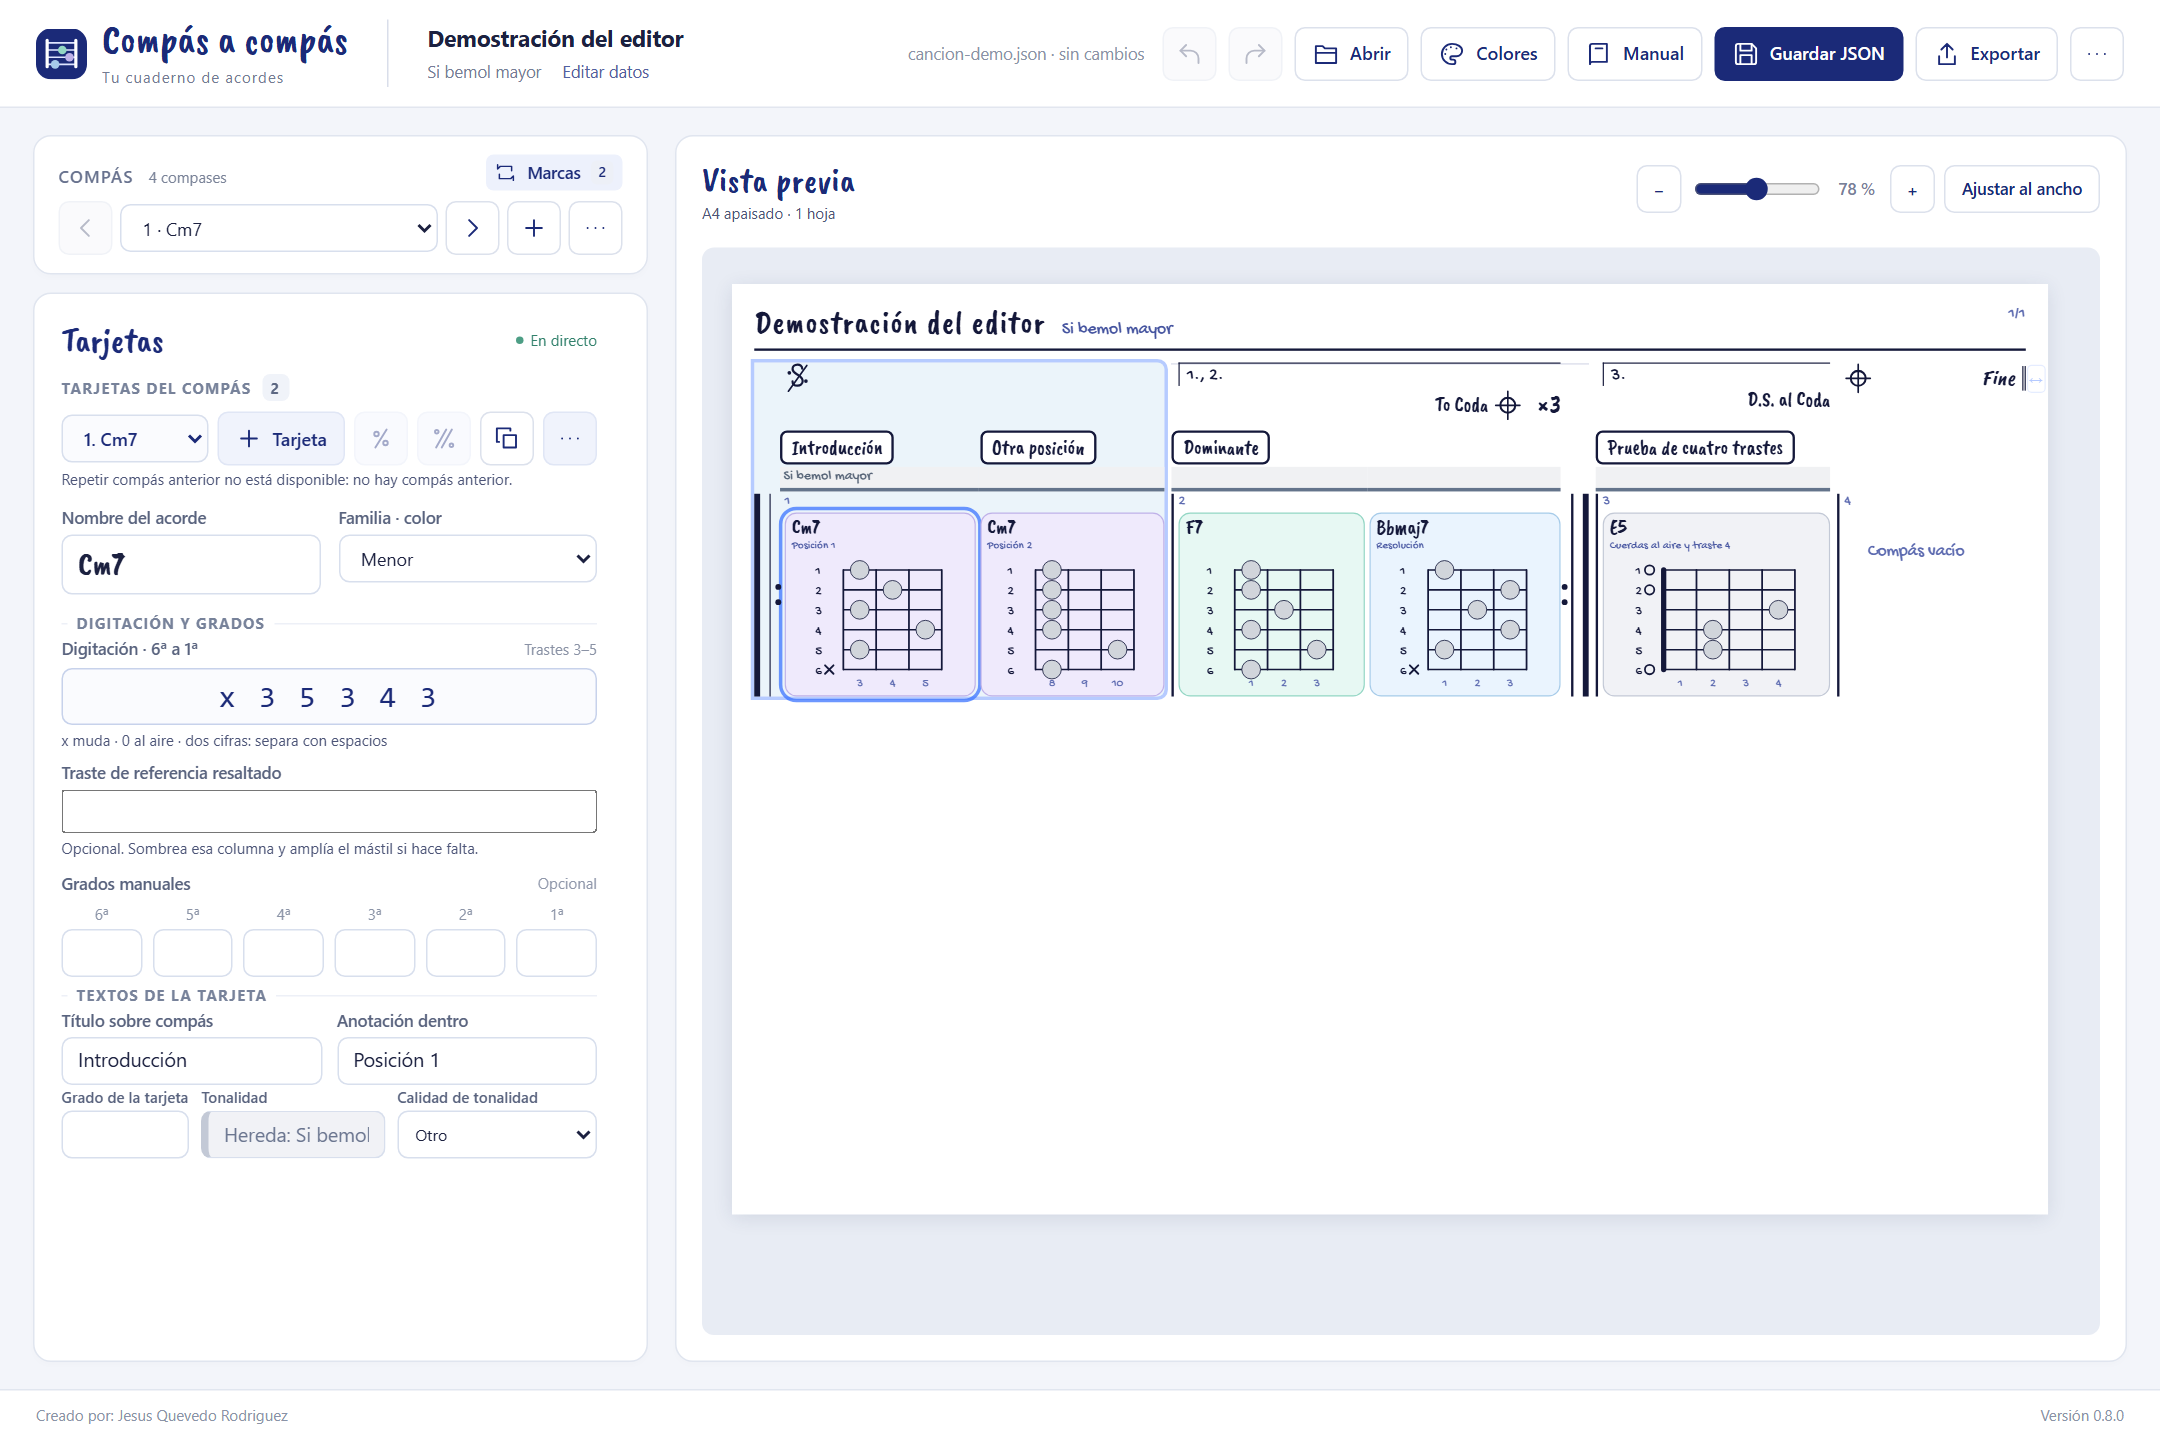
\includegraphics[width=\linewidth,height=0.44\textheight,keepaspectratio]{../manuals/capturas/editor-general.png}

\Needspace{3.5cm}
\hypertarget{tarjetas-del-compuxe1s}{%
\section{Tarjetas del compás}\label{tarjetas-del-compuxe1s}}

Cada dibujo es una \textbf{tarjeta}. Tiene su nombre de acorde,
calidad/color, digitación, grados, título exterior, anotación y
tonalidad. Para escribir dos digitaciones del mismo acorde, añade dos
tarjetas con ese nombre. Para escribir dos acordes distintos, cambia el
nombre de cada una. Se manejan igual.

Usa el único selector \textbf{Tarjetas del compás} para elegir una
tarjeta, o púlsala directamente en la hoja. \textbf{Añadir tarjeta} crea
una tarjeta lista para introducir sus notas y sin nombre: la hoja no
dibuja nada hasta que lo escribas (el editor muestra «Sin nombre» solo
como ayuda). \textbf{Duplicar tarjeta} copia la seleccionada a
continuación; \textbf{Quitar tarjeta} borra solamente esa tarjeta, tras
confirmar. Al editar un campo no cambian las otras tarjetas, aunque
compartan el mismo nombre.

Los archivos anteriores siguen abriendo. Si contenían varias posiciones
agrupadas bajo un acorde, ahora aparecen como tarjetas separadas en el
selector. Abrir y guardar sin editar conserva el archivo; el cambio de
interfaz no elimina datos ni crea notas.

Selecciona un compás en el desplegable superior o con las flechas. El
botón + añade un compás y el menú de tres puntos permite insertar,
duplicar, mover o borrar compases. Su etiqueta no se renumera
automáticamente al moverlos. Antes de borrar un compás se muestran las
consecuencias para sus marcas musicales.

\hypertarget{repetir-uno-o-dos-compases}{%
\subsection{Repetir uno o dos
compases}\label{repetir-uno-o-dos-compases}}

Junto a \textbf{Añadir tarjeta} hay dos botones con el signo de
repetición. No crean compases nuevos por sí solos ni copian tarjetas: la
hoja dibuja un signo grande y el contenido se lee en el origen.

\begin{itemize}
\tightlist
\item
  \textbf{Repetir compás anterior} (signo de porcentaje musical): el
  compás seleccionado repite el compás inmediatamente anterior. Está
  desactivado en el primer compás. Si el compás tiene tarjetas, pide
  confirmar antes de sustituirlas; cancelar no cambia nada y aceptar se
  deshace de una vez. Se permiten varios compases de repetición
  seguidos.
\item
  \textbf{Repetir dos compases anteriores} (dos barras oblicuas): el
  compás seleccionado y el siguiente forman la pareja de destino y
  repiten, en orden, los dos compases escritos antes. El signo se dibuja
  sobre la barra de compás común y los dos destinos van siempre en la
  misma línea. Necesita dos compases antes del seleccionado y uno
  después: si falta el segundo destino, la aplicación pregunta antes de
  añadir un compás vacío al final.
\end{itemize}

En un compás de repetición, el editor muestra un aviso con
\textbf{Quitar repetición} (en la pareja quita las dos a la vez y deja
ambos compases vacíos y editables). Si pulsas \textbf{Añadir tarjeta} en
uno de ellos, se sale de la repetición y se avisa. Números, Coda, Fine,
casillas y barras de repetición del compás se conservan.

Si borras o mueves un compás de origen o de destino, la referencia se
conserva y se avisa en el editor del compás y al mover; no se redirige
sola. \textbf{Corregir referencia} la apunta de nuevo a los compases
inmediatamente anteriores. Duplicar un compás de repetición hace que la
copia repita el original; duplicar un destino de una pareja crea un
compás vacío (y la pareja queda avisada si la copia la separa).

Los archivos con estos campos (\texttt{repeatPrevious},
\texttt{repeatPreviousTwo}) requieren 0.7.0 o posterior.

\Needspace{3.5cm}
\hypertarget{escribir-digitaciones-grados-y-textos}{%
\section{Escribir digitaciones, grados y
textos}\label{escribir-digitaciones-grados-y-textos}}

\hypertarget{digitaciuxf3n}{%
\subsection{Digitación}\label{digitaciuxf3n}}

Introduce \textbf{seis valores, de sexta a primera cuerda}: la cuerda
grave primero y la aguda al final. Usa \texttt{x} para una cuerda muda y
\texttt{0} para una cuerda al aire.

\begin{verbatim}
x 3 5 3 4 3       Cm7
x 10 12 10 11 10  Una posición en trastes de dos cifras
0 2 2 4 0 0       Ejemplo que ocupa cuatro trastes
\end{verbatim}

También se acepta \texttt{x35343} cuando cada traste tiene una cifra.
Usa espacios si hay trastes de dos cifras. Una entrada incorrecta
muestra un aviso y conserva la última digitación válida.

Una tarjeta nueva empieza con todas las cuerdas mudas: debes introducir
sus notas. En el dibujo, la primera cuerda está arriba. El mástil
muestra al menos tres trastes y \textbf{crece solo} a cuatro o más si lo
necesita. El límite actual es un intervalo visible de 32 trastes; si se
supera, conserva los datos, avisa y bloquea la exportación hasta
corregirlo.

\hypertarget{grados-y-color}{%
\subsection{Grados y color}\label{grados-y-color}}

Los seis campos de grados siguen el mismo orden, de sexta a primera
cuerda. Son opcionales y manuales: puedes escribir \texttt{1},
\texttt{b3}, \texttt{5} o \texttt{b7}, por ejemplo. Los grados
reconocidos colorean los puntos; un campo vacío deja la nota sin grado.
Los textos largos se abrevian en el punto y se explican en una leyenda.

El selector de calidad cambia el fondo de la tarjeta. No analiza sus
notas ni genera una digitación.

\hypertarget{elegir-los-colores}{%
\subsection{Elegir los colores}\label{elegir-los-colores}}

Pulsa \textbf{Colores} en la cabecera. En \textbf{Calidad del acorde}
cambia el fondo de mayor, menor, dominante, semidisminuido, disminuido y
otros. Se usa la familia que hayas elegido en cada acorde; no se deduce
del nombre.

En \textbf{Notas y grados}, elige naturales, bemoles o sostenidos para
ver los grados del 1 al 13. Cada uno tiene su propio color: cambiar
\texttt{b3} no modifica \texttt{3}. Puedes usar el selector de color o
escribir un hexadecimal \texttt{\#RRGGBB}. \textbf{Otro grado o
etiqueta} añade valores como \texttt{bb7}, \texttt{\#\#4} o \texttt{R},
de hasta 32 caracteres. Los símbolos ♭ y ♯ equivalen a \texttt{b} y
\texttt{\#}. Cada grado tiene un \textbf{Fondo} y un \textbf{Texto}
independientes (selector y hexadecimal, cada uno con su flecha de
restaurar); el texto es blanco por defecto y nunca se cambia solo. La
muestra enseña la combinación real. También se pueden cambiar el fondo y
el texto de las notas sin grado o sin un color propio; su fondo de serie
es un gris claro (\texttt{\#d1d5db}).

Las muestras se actualizan y los colores se aplican a todos los compases
de esta canción. En las tarjetas, el texto y la rejilla se adaptan para
leer sobre fondos oscuros; en los puntos de grado manda el texto que
elijas. La flecha circular restaura un color; \textbf{Restaurar paleta
original} pide confirmar antes de quitar todos los colores
personalizados.

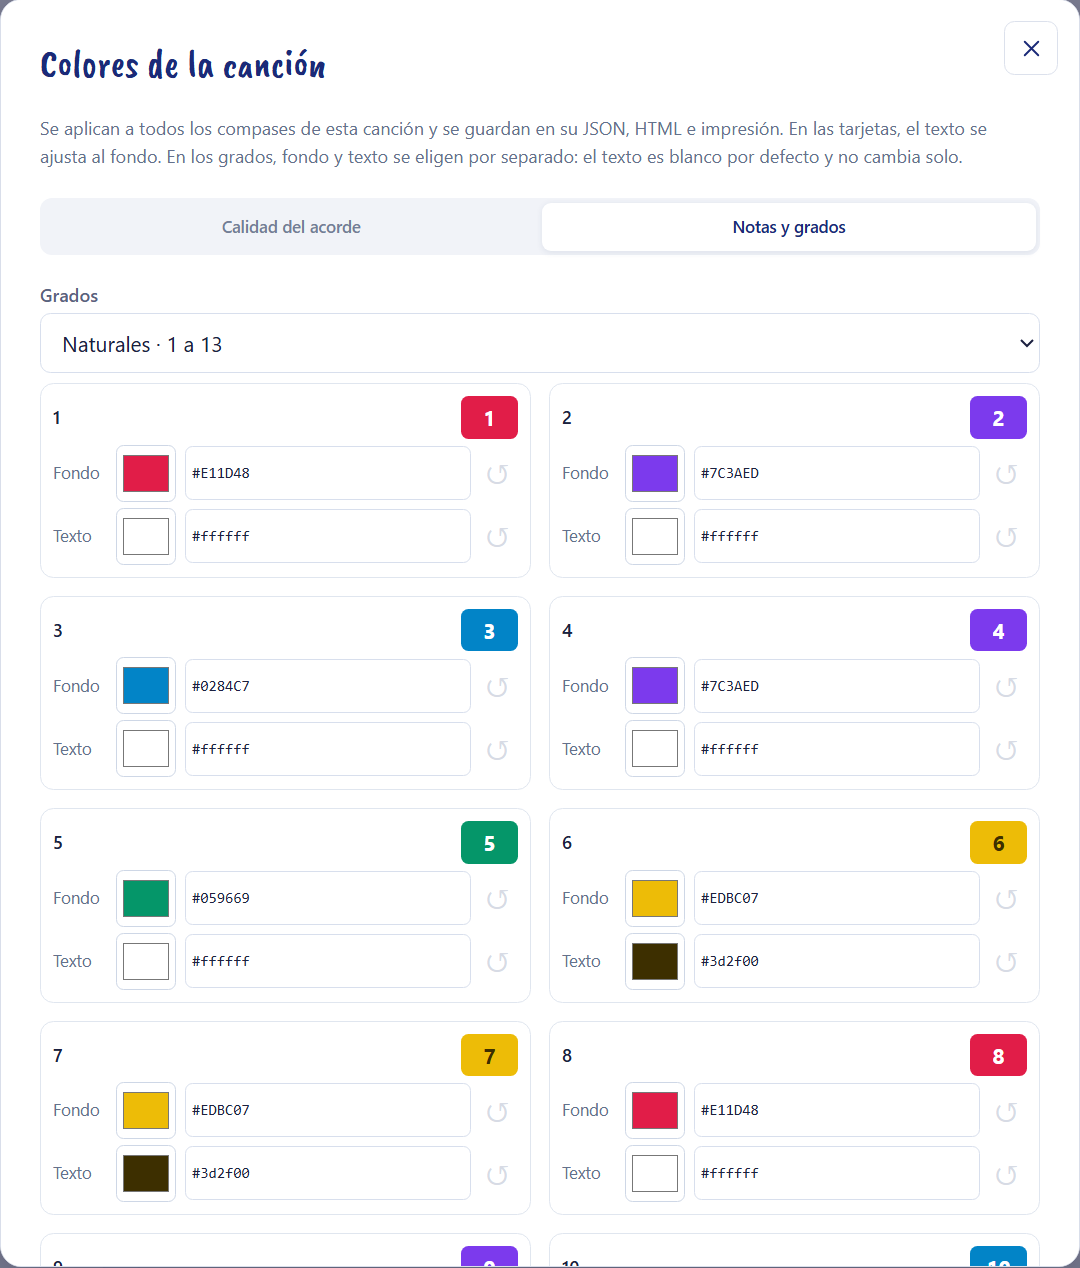
\includegraphics[width=\linewidth,height=0.44\textheight,keepaspectratio]{../manuals/capturas/colores-grados.png}

Pulsa \textbf{Listo} para cerrar y \textbf{Guardar JSON} para conservar
la paleta en el archivo. Se incluye también en HTML e impresión. Abrir
otra canción utiliza sus colores, o los predeterminados
(\texttt{config/palette-defaults.json}) si no tiene una paleta guardada;
esos valores nunca se escriben en tu archivo. Las versiones anteriores a
0.3.0 no pueden abrir JSON con el campo \texttt{palette}; utiliza la
aplicación actualizada.

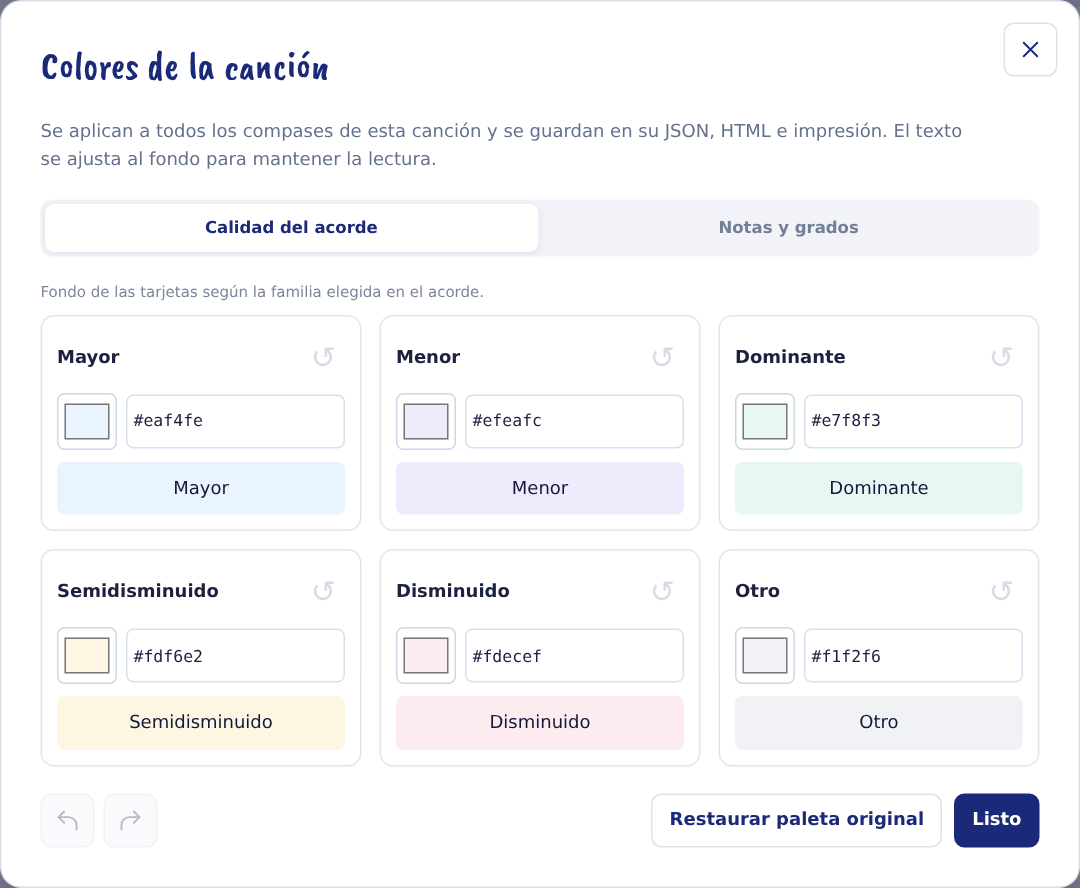
\includegraphics[width=\linewidth,height=0.44\textheight,keepaspectratio]{../manuals/capturas/colores-acordes.png}

\hypertarget{tuxedtulos-anotaciones-y-grado-de-la-tarjeta}{%
\subsection{Títulos, anotaciones y grado de la
tarjeta}\label{tuxedtulos-anotaciones-y-grado-de-la-tarjeta}}

El bloque \textbf{Textos de la tarjeta} aparece debajo de digitación y
grados, siempre visible y sin pestañas. \textbf{Título sobre la tarjeta}
se dibuja en un recuadro encima de su posición y fuera de la línea
vertical del compás. \textbf{Anotación dentro} conserva su lugar bajo el
nombre del acorde. Vaciar cualquiera lo quita de esa tarjeta.

Cada campo modifica solo la tarjeta seleccionada. No hay un selector
para aplicar los textos a otras tarjetas.

\textbf{Grado de la tarjeta} es un campo manual independiente: escribe
\texttt{ii}, \texttt{V7/ii} o el texto que necesites. Sale arriba a la
derecha de la tarjeta, junto al acorde. No modifica los seis grados de
las cuerdas ni se calcula automáticamente. Este campo pertenece siempre
a la posición seleccionada.

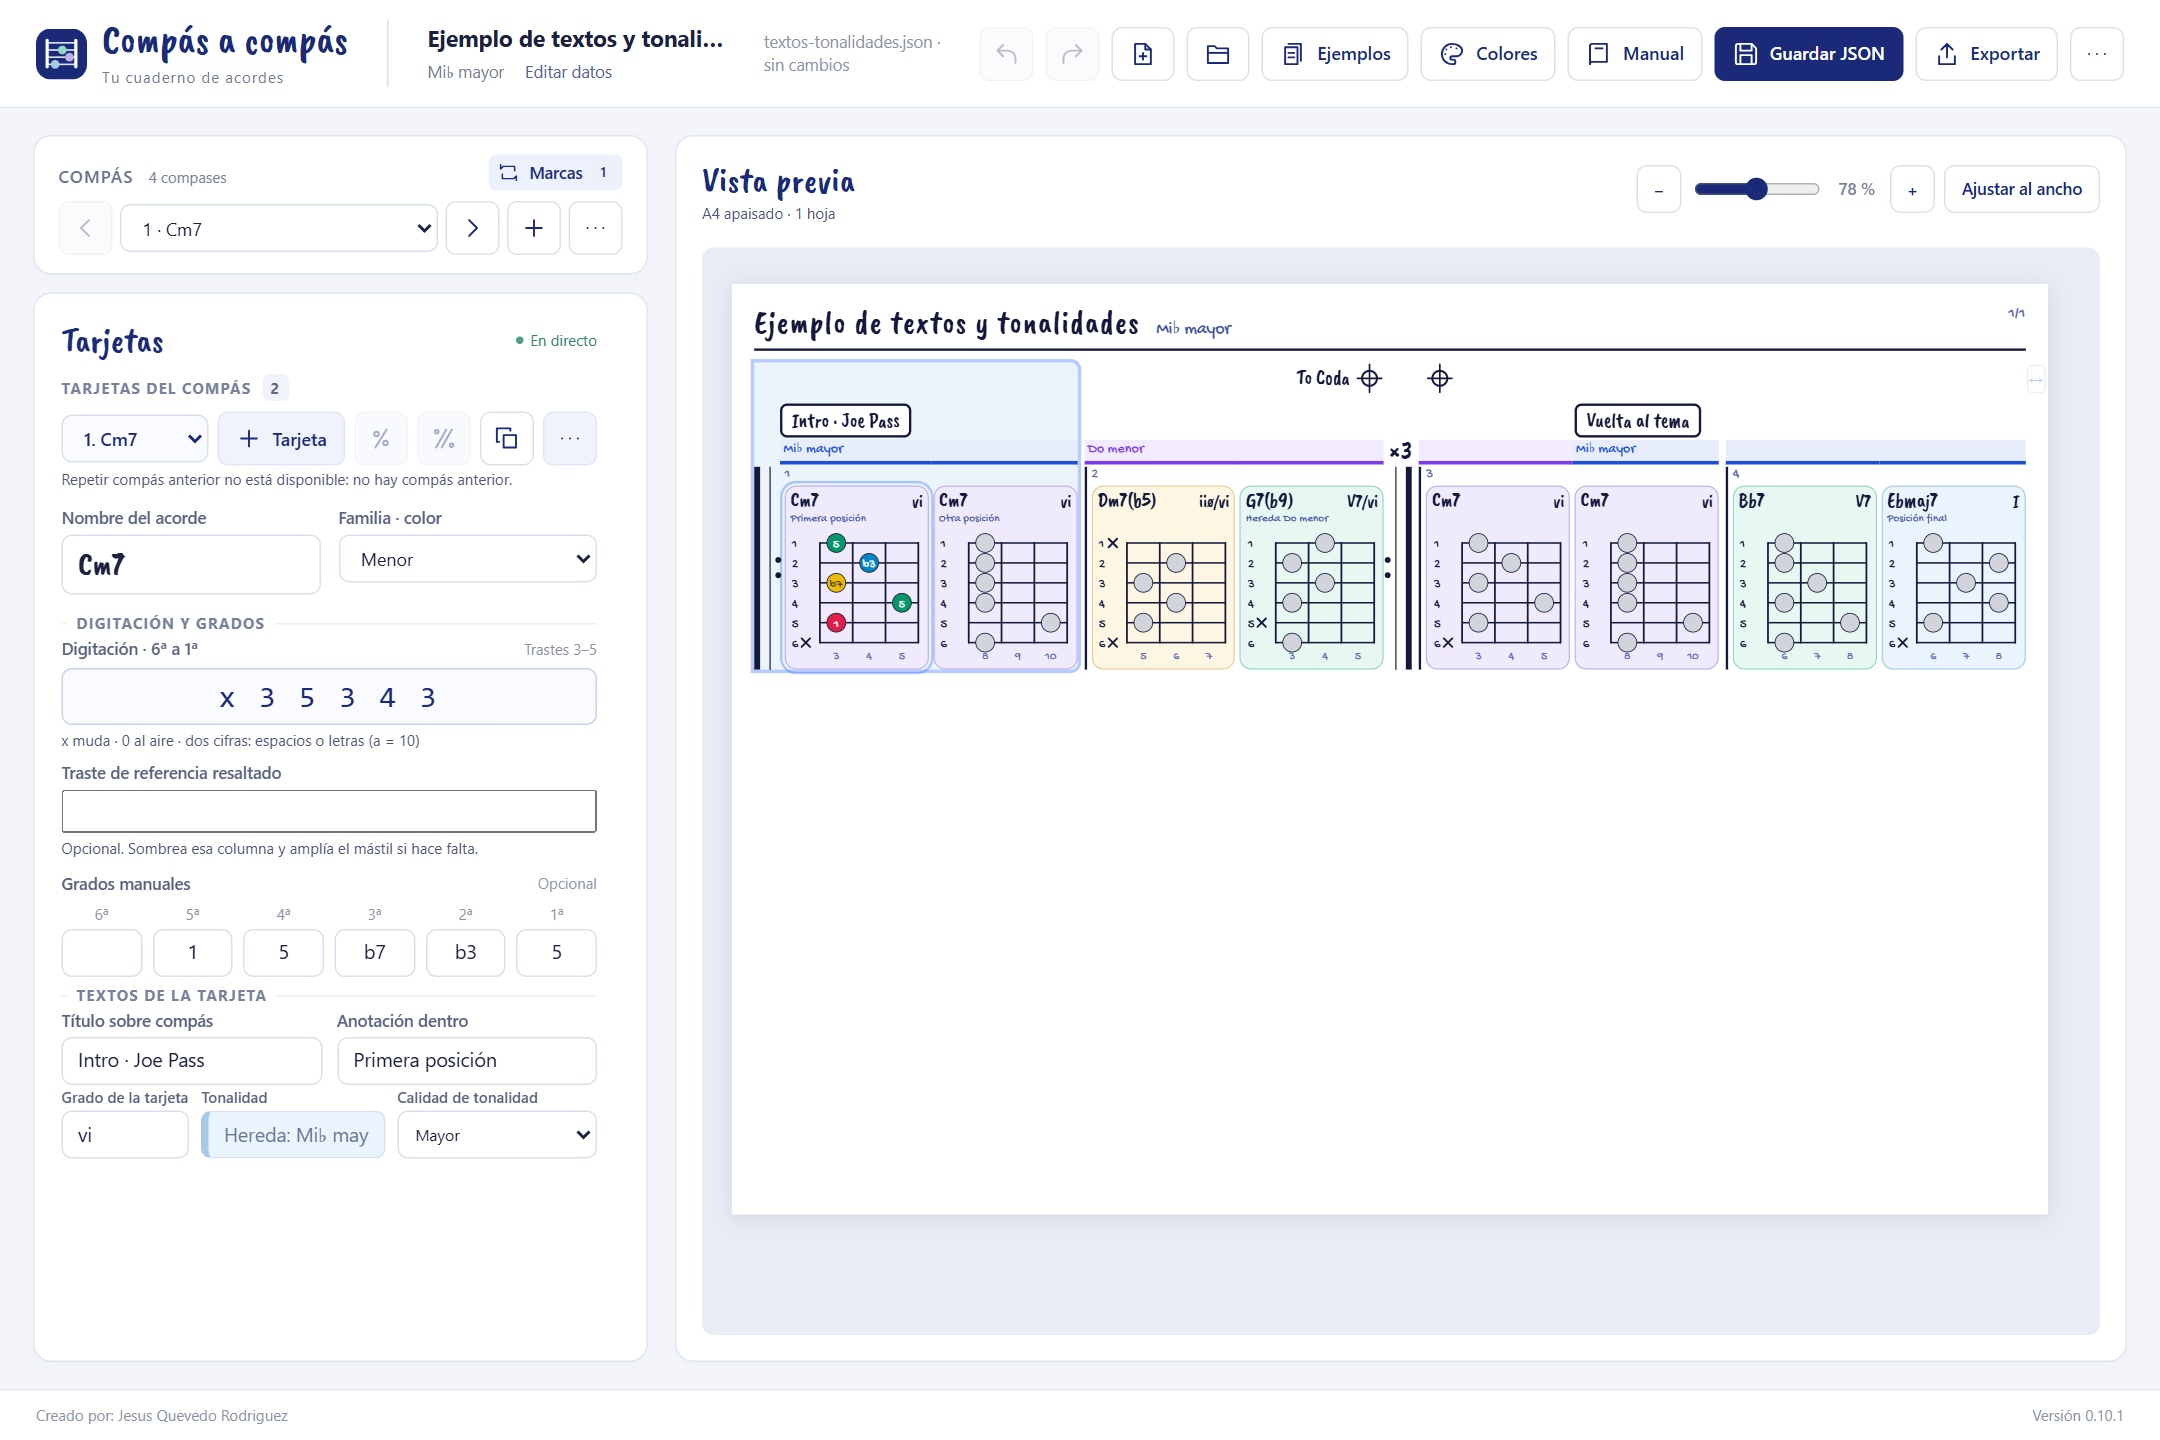
\includegraphics[width=\linewidth,height=0.44\textheight,keepaspectratio]{../manuals/capturas/textos-deshacer.png}

\hypertarget{tonalidad-de-cada-tarjeta}{%
\subsection{Tonalidad de cada tarjeta}\label{tonalidad-de-cada-tarjeta}}

En \textbf{Tonalidad} escribe un cambio de contexto y elige su
\textbf{Calidad de tonalidad}. Mayor, menor y las demás calidades usan
los colores de la paleta de familias de esta canción. La calidad de la
franja es independiente de la del acorde: un dominante puede llevar una
tonalidad menor encima. La banda es rectangular, con fondo tenue y línea
de color debajo, como en la plantilla; no lleva recuadro redondeado.

Deja el campo vacío para continuar con la tonalidad anterior, incluido
su color, sin imprimir otra etiqueta. La herencia sigue el orden escrito
a través de acordes, compases y páginas. No interpreta las repeticiones.
Borrar un cambio hace que esa posición y las siguientes vuelvan a
heredar del contexto anterior, hasta el próximo cambio escrito.

La tonalidad general inicia el contexto; si no has elegido su calidad,
usa el color neutro de \textbf{Otro}. Sin tonalidad general ni cambio
previo no se inventa ninguna. Cuando está vacío, el campo muestra una
guía «Hereda: \ldots» y el color del contexto efectivo; al pasar el
ratón se ve la explicación completa. Elegir una calidad con el campo
vacío prepara el siguiente texto; no crea un cambio invisible en el
archivo.

Para ocultar las franjas en todas las hojas, abre los datos de canción
pulsando su título y desmarca \textbf{Mostrar tonalidades de las
tarjetas}. La tonalidad junto al título sigue visible. Mientras estén
ocultas, los campos \textbf{Tonalidad} y \textbf{Calidad de tonalidad}
de cada tarjeta también desaparecen del editor, porque no tendrían
efecto en la hoja; sus valores se conservan y reaparecen al volver a
marcar la casilla. No se borra ningún dato.

Grado y tonalidad pertenecen a la tarjeta seleccionada, igual que el
resto de sus campos. Se guardan en JSON y se conservan en vista previa,
HTML e impresión. Puedes probarlo abriendo
\texttt{examples/textos-tonalidades.json}. Los archivos con estos campos
nuevos requieren 0.5.0 o posterior; los anteriores siguen abriendo.

\hypertarget{deshacer-y-rehacer}{%
\subsection{Deshacer y rehacer}\label{deshacer-y-rehacer}}

Pulsa la flecha hacia la izquierda de la cabecera para \textbf{Deshacer}
y la flecha hacia la derecha para \textbf{Rehacer}. También están dentro
de los diálogos de datos, marcas y colores, por lo que puedes deshacer
una coda sin cerrar su panel. Se deshacen las acciones aplicadas a la
canción: textos, digitaciones, grados, tonalidades, su visibilidad,
colores, compases, acordes, posiciones y marcas musicales.

La escritura continua en un campo se agrupa hasta salir de él. Fuera de
los campos funcionan \textbf{Ctrl+Z} y \textbf{Ctrl+Y} o
\textbf{Ctrl+Mayús+Z}; en Mac se puede usar Cmd. Dentro de un campo se
conserva el deshacer habitual del navegador, también para los borradores
de marcas que todavía no se han añadido.

Guardar JSON conserva el historial de esta sesión. Abrir otra canción,
crear una nueva o recuperar una copia empieza otro historial. Al
recargar se conserva la canción que ofrezca la recuperación, pero no sus
pasos de deshacer. Hay hasta 100 pasos, sujetos a un presupuesto de
tamaño; la última acción siempre se conserva. El historial no se incluye
en el JSON. Una acción nueva después de deshacer elimina la rama de
rehacer.

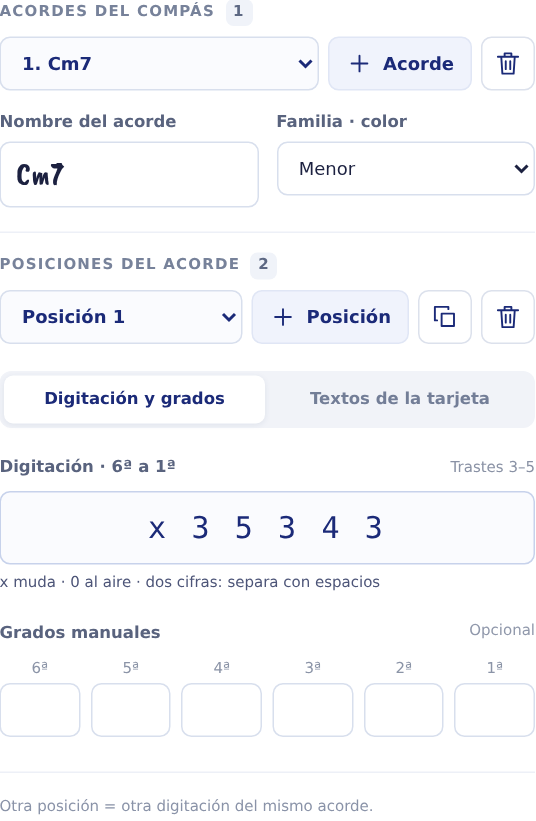
\includegraphics[width=\linewidth,height=0.44\textheight,keepaspectratio]{../manuals/capturas/editor-posiciones.png}

\hypertarget{opciones-de-puxe1gina}{%
\subsection{Opciones de página}\label{opciones-de-puxe1gina}}

En los datos de canción hay opciones globales que solo cambian la
presentación:

\begin{itemize}
\tightlist
\item
  \textbf{Máximo de compases por línea}: \textbf{Automático} (por
  defecto) reparte según el ancho disponible, como siempre. Un número
  del 1 al 16 es un tope, no una obligación: pueden caber menos compases
  si las tarjetas son anchas o la pantalla estrecha. La pareja de una
  repetición de dos compases no se separa, así que con tope 1 ocupa una
  línea con sus dos compases.
\item
  \textbf{Mostrar números de compás}: al desmarcarla se ocultan las
  etiquetas de todos los compases y las líneas verticales que los
  separan, en la vista previa, el HTML y la impresión, útil para una
  hoja de acordes que no es una partitura. Las etiquetas se conservan en
  el archivo. Las líneas de las tarjetas, las barras y signos de
  repetición, Coda, Fine, casillas, saltos y el número de página siguen
  visibles.
\item
  \textbf{Tamaño de los mástiles}: reduce proporcionalmente los
  diagramas para que quepan más filas por página, sin cambiar trastes ni
  notas. El 100 \% conserva el tamaño normal.
\end{itemize}

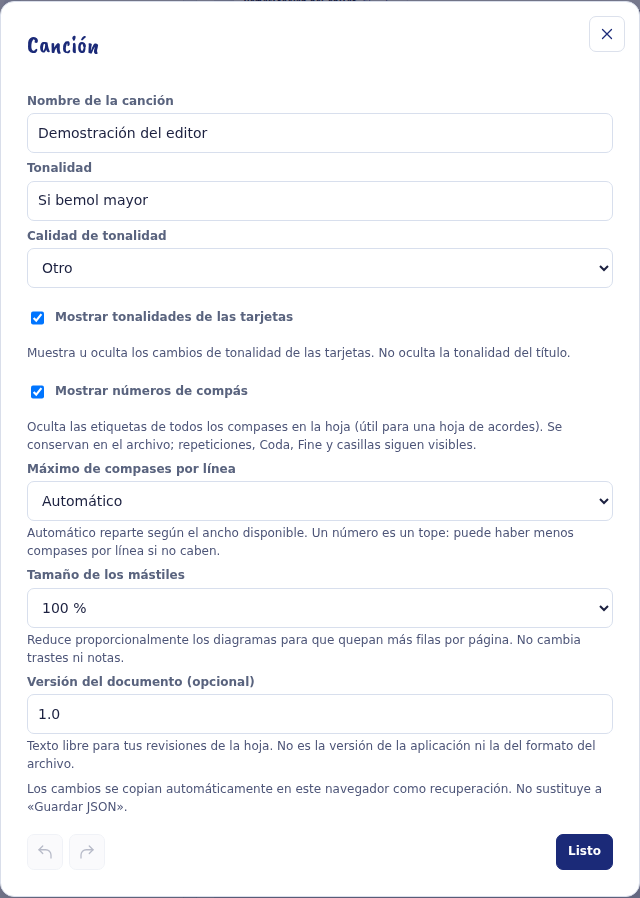
\includegraphics[width=\linewidth,height=0.44\textheight,keepaspectratio]{../manuals/capturas/datos-cancion.png}

Las opciones se guardan en el JSON cuando tienen un valor distinto del
predeterminado. Las versiones anteriores a la que incorpora
\texttt{fretboardScalePercent} no abren archivos que incluyan ese campo.

\hypertarget{ancho-de-cada-compuxe1s-y-ajuste-de-luxednea}{%
\subsection{Ancho de cada compás y ajuste de
línea}\label{ancho-de-cada-compuxe1s-y-ajuste-de-luxednea}}

\begin{itemize}
\tightlist
\item
  \textbf{Ancho del compás}: en el menú de tres puntos del compás,
  escribe un porcentaje del 10 al 100 \% del ancho de la línea. Vacío es
  Automático (como siempre). El ancho nunca baja de lo que necesitan las
  tarjetas: si el porcentaje no basta se usa el mínimo, aparece un aviso
  bajo la vista previa y caben menos compases en esa línea.
\item
  \textbf{Ajustar línea al ancho}: cada línea de la vista previa tiene
  un botón de doble flecha horizontal en el margen derecho de la hoja.
  Al pulsarlo, el espacio libre se reparte entre los compases de esa
  línea hasta el margen derecho, sin deformar los mástiles ni comprimir
  ninguna tarjeta, y puede superar el 25 \%. Pulsa de nuevo (queda
  resaltado) para volver a Automático, o usa Deshacer. Si la línea
  cambia de composición, el reparto se recalcula con los compases que
  caben.
\end{itemize}

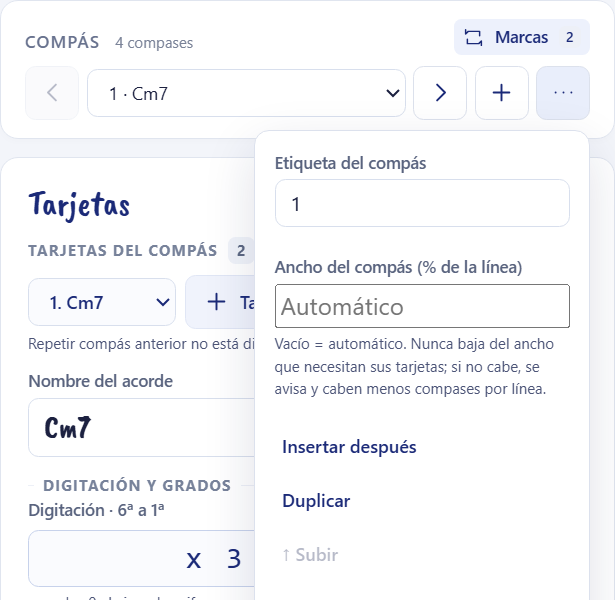
\includegraphics[width=\linewidth,height=0.44\textheight,keepaspectratio]{../manuals/capturas/opciones-compas.png}

Ambos ajustes se guardan en el JSON solo cuando se usan
(\texttt{widthPercent}, \texttt{fillToEdge}); las versiones anteriores a
0.7.0 no abren esos archivos.

Al ajustar al ancho varias filas de una misma página con la misma
estructura, las tarjetas se alinean verticalmente. El reparto común
respeta el ancho mínimo que necesita cada tarjeta; si no hay espacio
suficiente para alinear sin comprimir contenido, se mantienen los anchos
individuales.

Las filas ya no se estiran a todo el ancho: cada tarjeta crece como
mucho un 25 \% sobre su ancho natural y el sobrante queda a la derecha.

\Needspace{3.5cm}
\hypertarget{auxf1adir-varios-compases-mediante-una-lista}{%
\section{Añadir varios compases mediante una
lista}\label{auxf1adir-varios-compases-mediante-una-lista}}

Abre el menú de tres puntos del bloque Compás y pulsa \textbf{Importar
lista} e introduce una línea por compás:

\begin{verbatim}
1 | Cm7 @ x 3 5 3 4 3 / 8 10 8 8 8 8
2 | F7 @ 1 3 1 2 1 1 ; Bbmaj7 @ x 1 3 2 3 1
3 |
\end{verbatim}

\begin{itemize}
\tightlist
\item
  \texttt{\textbar{}} separa la etiqueta y el contenido del compás.
\item
  \texttt{@} separa el nombre del acorde y su digitación.
\item
  \texttt{;} añade otro acorde al mismo compás.
\item
  \texttt{/}, con espacios, añade otra posición al acorde. \texttt{C/E}
  sigue siendo un nombre de acorde.
\item
  Una línea como \texttt{3\ \textbar{}} crea un compás vacío.
\end{itemize}

Comprueba la previsualización. La lista se \textbf{añade al final} de la
canción y solo se importa si no hay errores. No sustituye los compases
existentes.

\Needspace{3.5cm}
\hypertarget{repeticiones-casillas-y-saltos}{%
\section{Repeticiones, casillas y
saltos}\label{repeticiones-casillas-y-saltos}}

Pulsa \textbf{Marcas}, junto al selector del compás. El título del panel
indica \textbf{Marcas del compás 4}, por ejemplo. Muestra las marcas
escritas en ese compás y las repeticiones o casillas cuyo tramo lo
incluye.

Al cambiar de compás, también desde el selector del propio panel, las
nuevas marcas parten del elegido. Las marcas ya guardadas conservan su
ubicación. Si estabas rellenando una marca sin guardar, cambiar de
compás prepara un formulario nuevo; pulsa \textbf{Añadir marca} o
\textbf{Guardar cambios} antes si quieres conservar esa edición.

\textbf{Ver todas las marcas} muestra el conjunto de la canción,
incluidas referencias pendientes que no puedan asociarse a un compás
existente. \textbf{Ver este compás} vuelve al filtro local. Los avisos
pendientes de toda la canción permanecen visibles.

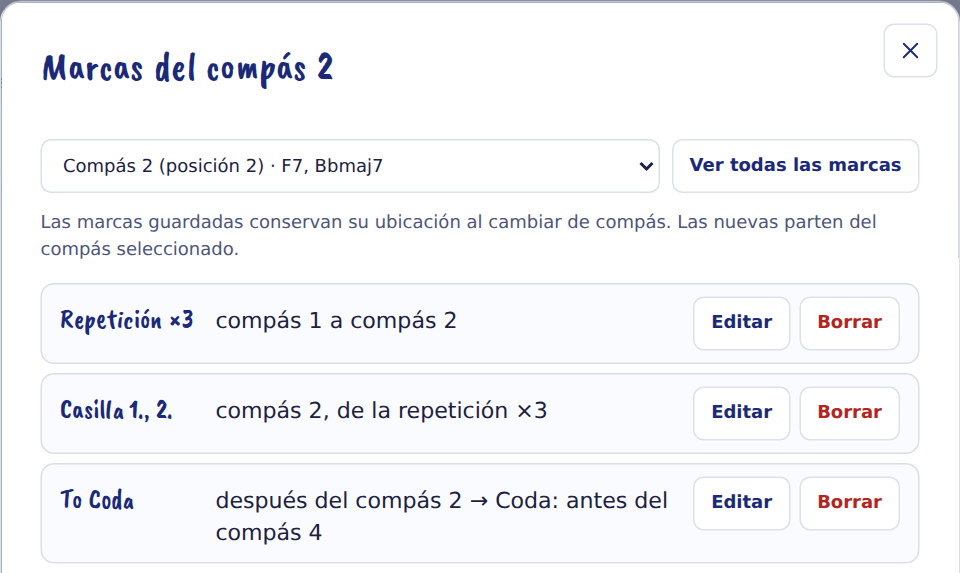
\includegraphics[width=\linewidth,height=0.44\textheight,keepaspectratio]{../manuals/capturas/marcas-compas.png}

El formulario permite añadir y editar la estructura escrita:

\begin{longtable}[]{@{}>{\raggedright\arraybackslash}p{\dimexpr0.320000\linewidth-1.000000\tabcolsep\relax}>{\raggedright\arraybackslash}p{\dimexpr0.680000\linewidth-1.000000\tabcolsep\relax}@{}}
\toprule\noalign{}
Marca & Cómo prepararla \\
\midrule\noalign{}
\endhead
\bottomrule\noalign{}
\endlastfoot
Repetición & Elige el compás inicial, el final y el número total de
pasadas. ×3 significa tres pasadas en total. \\
Casilla & Elige su inicio y final, las pasadas y, cuando corresponda, la
repetición a la que pertenece. \\
Segno, Coda y Fine & Coloca la marca antes o después del compás
elegido. \\
D.C., D.S. y variantes & Elige el salto y los destinos Segno, Coda o
Fine que solicite el formulario. \\
To Coda & Colócalo en el punto de salida y selecciona la Coda de
destino. \\
\end{longtable}

Para una indicación \textbf{D.S. al Coda}, crea primero el Segno y la
Coda; después configura el salto y el To Coda correspondiente. Revisa el
recorrido escrito como lo harías en una partitura.

Las marcas se dibujan, pero \textbf{no hay reproducción ni comprobación
del recorrido musical completo}. Si falta un destino, aparece un aviso y
la referencia queda pendiente; no salta a otro compás por su cuenta.
Corrige el destino desde el panel. Antes de exportar referencias
pendientes se pide confirmación.

\Needspace{3.5cm}
\hypertarget{guardar-y-recuperar-el-trabajo}{%
\section{Guardar y recuperar el
trabajo}\label{guardar-y-recuperar-el-trabajo}}

\textbf{Guardar JSON} conserva la canción editable completa. Según el
navegador, aparecerá un selector de archivo o una descarga. Elige una
carpeta conocida y conserva copias con nombres como
\texttt{Mi-cancion-01.json}.

\textbf{Abrir JSON} permite continuar ese proyecto. Si el formato es
inválido, tiene campos desconocidos o pertenece a otra versión de
esquema, se rechaza y la canción abierta se conserva. Nuevo y Abrir
avisan si tienes cambios pendientes.

El navegador guarda además una recuperación local y la ofrece al volver
a entrar si quedaron cambios pendientes. Depende del mismo navegador,
perfil y dirección de la aplicación; otro puerto usa otro
almacenamiento. Se borra al guardar, abrir o crear una canción.
\textbf{La recuperación no sustituye al archivo JSON.}

Exportar HTML o imprimir no equivale a guardar los cambios del proyecto.
Guarda el JSON antes de cerrar. Deshacer permite corregir acciones de
esta sesión; no sustituye al archivo guardado.

\Needspace{3.5cm}
\hypertarget{exportar-e-imprimir}{%
\section{Exportar e imprimir}\label{exportar-e-imprimir}}

Abre el menú \textbf{Exportar} de la cabecera. \textbf{Exportar HTML}
crea un archivo único con las hojas, estilos y fuentes incluidos. Puedes
abrirlo sin conexión y compartirlo. No contiene el editor ni sirve para
recuperar una canción editable.

\textbf{Imprimir / PDF} abre la impresión del navegador con las mismas
hojas. Para guardar como PDF:

\begin{enumerate}
\def\labelenumi{\arabic{enumi}.}
\tightlist
\item
  Selecciona \textbf{Guardar como PDF} como destino.
\item
  Elige papel \textbf{A4 horizontal}, escala \textbf{100 \%} y márgenes
  \textbf{Ninguno}.
\item
  Desactiva los encabezados y pies del navegador. Activa los gráficos de
  fondo si los colores no aparecen.
\item
  Revisa la previsualización y guarda el archivo.
\end{enumerate}

Cada página lleva nombre de canción, tonalidad y numeración
\texttt{actual/total} arriba a la derecha. La hoja mide 297 × 210 mm y
ya incluye sus márgenes de 5 mm.

Las filas se adaptan al contenido: no hay cuatro compases fijos por
fila. Al añadir compases se vuelve a repartir la canción. Las tarjetas
pueden ensancharse para completar una fila, mientras el dibujo conserva
la escala de sus trastes. Un compás muy largo continúa entre tarjetas en
otra fila u hoja, con su etiqueta y la indicación de continuación.

Si una digitación o un bloque no cabe, se avisa y se bloquea la salida;
nunca se modifican tus trastes para hacerlos caber.

\Needspace{3.5cm}
\hypertarget{si-algo-no-sale-como-esperabas}{%
\section{Si algo no sale como
esperabas}\label{si-algo-no-sale-como-esperabas}}

\begin{longtable}[]{@{}>{\raggedright\arraybackslash}p{\dimexpr0.320000\linewidth-1.000000\tabcolsep\relax}>{\raggedright\arraybackslash}p{\dimexpr0.680000\linewidth-1.000000\tabcolsep\relax}@{}}
\toprule\noalign{}
Situación & Qué revisar \\
\midrule\noalign{}
\endhead
\bottomrule\noalign{}
\endlastfoot
He añadido una posición y parece vacía & Empieza con seis cuerdas mudas.
Escribe una digitación distinta para verla. \\
Dos tarjetas muestran el mismo texto & Selecciona una y edita sus
textos; solo cambia esa tarjeta. \\
La siguiente hoja tiene tarjetas más anchas & Las filas parciales
reparten el ancho disponible. El zoom no cambia el tamaño exportado. \\
El grado no aparece & Comprueba el orden de las cuerdas y si esa cuerda
está muda. \\
Hay un destino pendiente & Vuelve a elegir la marca o el compás en el
panel Marcas. \\
El navegador no abre la aplicación & Abre GitHub Pages o arranca el
servidor local; consulta la guía de instalación. \\
\end{longtable}
\end{document}
